\documentclass[12pt, french]{report}
% -----------------------------
% Devoir : ACT-2009
% -----------------------------
\title{Devoir}
\date{\today}
% -----------------------------
% Préambule
% !TEX encoding = UTF-8 Unicode
% LaTeX Preamble
% Author : Gabriel Crépeault-Cauchon
% Last update : 15/10/2018

% HOW-TO : copy-paste this file in the same directory as your .tex file, and add in your preamble the next command right after you have specified your documentclass : 
% % !TEX encoding = UTF-8 Unicode
% LaTeX Preamble
% Author : Gabriel Crépeault-Cauchon
% Last update : 15/10/2018

% HOW-TO : copy-paste this file in the same directory as your .tex file, and add in your preamble the next command right after you have specified your documentclass : 
% % !TEX encoding = UTF-8 Unicode
% LaTeX Preamble
% Author : Gabriel Crépeault-Cauchon
% Last update : 15/10/2018

% HOW-TO : copy-paste this file in the same directory as your .tex file, and add in your preamble the next command right after you have specified your documentclass : 
% \input{preambule_utf8.tex}
% ---------------------------------------------
% ---------------------------------------------
%% BEGINNING OF PREAMBLE
% Encoding packages
\usepackage[utf8]{inputenc}
\usepackage[T1]{fontenc}
\usepackage{babel}
\usepackage{lmodern}

% HYPERREF (URL's and Link options)
\usepackage{hyperref}
\hypersetup{colorlinks = true, urlcolor = blue, linkcolor = black}

% POLICY (choose one of them)
%	\usepackage{concrete}
%	\usepackage{mathpazo}
%	\usepackage{frcursive} %% permet d'écrire en lettres attachées
%	\usepackage{aeguill}
	\usepackage{mathptmx}
%	\usepackage{fourier} 

% Mathematics configuration
\usepackage{amsmath,amsthm,amssymb,latexsym,amsfonts}
\usepackage{empheq}
\usepackage{numprint}


% Tcolorbox config
\usepackage{tcolorbox}
\tcbuselibrary{xparse}
\tcbuselibrary{breakable}
%% Définition Boite pour exemple
\newcounter{ex}[section]
\DeclareTColorBox{exemple}{ o }% #1 parameter
{colframe=green!20!black,colback=green!5!white, % color of the box
breakable, pad at break*=0mm, % to split the box
before title = {\textbf{Exemple \stepcounter{ex} \arabic{chapter}.\arabic{section}.\arabic{ex} }},
IfValueTF = {#1}{title= {#1}}{title= \hphantom},
after title = {\large \hfill \faWrench}
}% conditionnal usage : if a title is specified, use it, else put "Exemple"

%% Définition boite pour définition
\newcounter{def}[section]
\DeclareTColorBox{definition}{ o }% #1 parameter
{colframe=blue!60!green,colback=blue!5!white, % color of the box
breakable, pad at break*=0mm, % to split the box
before title = {\textbf{Définition \stepcounter{def} \arabic{chapter}.\arabic{section}.\arabic{def} }},
title = {#1},
after title = {\large \hfill \faBook}
}


% Graphics and picture import Packages
\usepackage{graphicx}
\usepackage{pict2e}

% insert PDF package
\usepackage{pdfpages}

% Color package
\usepackage{color, soulutf8, colortbl}

% usefull shortcut for colored text
\newcommand{\orange}{\textcolor{orange}}
\newcommand{\red}{\textcolor{red}}
\newcommand{\cyan}{\textcolor{cyan}}
\newcommand{\blue}{\textcolor{blue}}
\newcommand{\green}{\textcolor{green}}
\newcommand{\purple}{\textcolor{magenta}}
\newcommand{\yellow}{\textcolor{yellow}}

% Custum enumerate & itemize Package
\usepackage{enumitem}
% Change default label for itemize
\renewcommand{\labelitemi}{\faAngleRight}

% Mathematics shortcut
\newcommand{\reels}{\mathbb{R}}
\newcommand{\entiers}{\mathbb{Z}}
\newcommand{\naturels}{\mathbb{N}}
\newcommand{\eval}{\biggr \rvert}
\usepackage{cancel}
\newcommand{\derivee}[1]{\frac{\partial}{\partial #1}}
\newcommand{\prob}[1]{\Pr \left( #1 \right)}
\newcommand{\esp}[1]{E \left[ #1 \right]}
\newcommand{\var}[1]{\text{Var} \left( #1 \right)}
\newcommand{\laplace}{\mathcal{L}}
\newcommand{\indic}[1]{\mathds{1}_{\{ #1 \}}}
\newcommand*\diff{\mathop{}\!\mathrm{d}}
\newcommand*\Diff[1]{\mathop{}\!\mathrm{d^#1}}

% To indicate equation number on a specific line in align environment
\newcommand\numberthis{\addtocounter{equation}{1}\tag{\theequation}}

% Actuarial notation package
\usepackage{actuarialsymbol}
\usepackage{actuarialangle}

% Other shortcut
\newcommand{\p}{\paragraph{}}
\newcommand{\n}{\newline}

% Special symbols package
\usepackage[tikz]{bclogo}
\usepackage{fontawesome}

% Chapter configuration
\setcounter{chapter}{0}
\setcounter{section}{0}

% LST
\usepackage{listings}
\usepackage{pdflscape}

% Retire l'indentation automatique
\setlength{\parindent}{0pt}

%% Configuration ajoutée pour le TP de modèles
%%%%%%%%
% pour xtable (entête rotationnée)
\usepackage{rotating}
\usepackage{makecell}

% Ajout pour changer les captions des tables pour qu'il affiche 'Tableau' (comme l'auto-ref ...)
\usepackage{caption}
\def\frenchtablename{TABLEAU}


%%%%%%%%




%% END OF PREAMBLE
% ---------------------------------------------
% ---------------------------------------------
% ---------------------------------------------
% ---------------------------------------------
%% BEGINNING OF PREAMBLE
% Encoding packages
\usepackage[utf8]{inputenc}
\usepackage[T1]{fontenc}
\usepackage{babel}
\usepackage{lmodern}

% HYPERREF (URL's and Link options)
\usepackage{hyperref}
\hypersetup{colorlinks = true, urlcolor = blue, linkcolor = black}

% POLICY (choose one of them)
%	\usepackage{concrete}
%	\usepackage{mathpazo}
%	\usepackage{frcursive} %% permet d'écrire en lettres attachées
%	\usepackage{aeguill}
	\usepackage{mathptmx}
%	\usepackage{fourier} 

% Mathematics configuration
\usepackage{amsmath,amsthm,amssymb,latexsym,amsfonts}
\usepackage{empheq}
\usepackage{numprint}


% Tcolorbox config
\usepackage{tcolorbox}
\tcbuselibrary{xparse}
\tcbuselibrary{breakable}
%% Définition Boite pour exemple
\newcounter{ex}[section]
\DeclareTColorBox{exemple}{ o }% #1 parameter
{colframe=green!20!black,colback=green!5!white, % color of the box
breakable, pad at break*=0mm, % to split the box
before title = {\textbf{Exemple \stepcounter{ex} \arabic{chapter}.\arabic{section}.\arabic{ex} }},
IfValueTF = {#1}{title= {#1}}{title= \hphantom},
after title = {\large \hfill \faWrench}
}% conditionnal usage : if a title is specified, use it, else put "Exemple"

%% Définition boite pour définition
\newcounter{def}[section]
\DeclareTColorBox{definition}{ o }% #1 parameter
{colframe=blue!60!green,colback=blue!5!white, % color of the box
breakable, pad at break*=0mm, % to split the box
before title = {\textbf{Définition \stepcounter{def} \arabic{chapter}.\arabic{section}.\arabic{def} }},
title = {#1},
after title = {\large \hfill \faBook}
}


% Graphics and picture import Packages
\usepackage{graphicx}
\usepackage{pict2e}

% insert PDF package
\usepackage{pdfpages}

% Color package
\usepackage{color, soulutf8, colortbl}

% usefull shortcut for colored text
\newcommand{\orange}{\textcolor{orange}}
\newcommand{\red}{\textcolor{red}}
\newcommand{\cyan}{\textcolor{cyan}}
\newcommand{\blue}{\textcolor{blue}}
\newcommand{\green}{\textcolor{green}}
\newcommand{\purple}{\textcolor{magenta}}
\newcommand{\yellow}{\textcolor{yellow}}

% Custum enumerate & itemize Package
\usepackage{enumitem}
% Change default label for itemize
\renewcommand{\labelitemi}{\faAngleRight}

% Mathematics shortcut
\newcommand{\reels}{\mathbb{R}}
\newcommand{\entiers}{\mathbb{Z}}
\newcommand{\naturels}{\mathbb{N}}
\newcommand{\eval}{\biggr \rvert}
\usepackage{cancel}
\newcommand{\derivee}[1]{\frac{\partial}{\partial #1}}
\newcommand{\prob}[1]{\Pr \left( #1 \right)}
\newcommand{\esp}[1]{E \left[ #1 \right]}
\newcommand{\var}[1]{\text{Var} \left( #1 \right)}
\newcommand{\laplace}{\mathcal{L}}
\newcommand{\indic}[1]{\mathds{1}_{\{ #1 \}}}
\newcommand*\diff{\mathop{}\!\mathrm{d}}
\newcommand*\Diff[1]{\mathop{}\!\mathrm{d^#1}}

% To indicate equation number on a specific line in align environment
\newcommand\numberthis{\addtocounter{equation}{1}\tag{\theequation}}

% Actuarial notation package
\usepackage{actuarialsymbol}
\usepackage{actuarialangle}

% Other shortcut
\newcommand{\p}{\paragraph{}}
\newcommand{\n}{\newline}

% Special symbols package
\usepackage[tikz]{bclogo}
\usepackage{fontawesome}

% Chapter configuration
\setcounter{chapter}{0}
\setcounter{section}{0}

% LST
\usepackage{listings}
\usepackage{pdflscape}

% Retire l'indentation automatique
\setlength{\parindent}{0pt}

%% Configuration ajoutée pour le TP de modèles
%%%%%%%%
% pour xtable (entête rotationnée)
\usepackage{rotating}
\usepackage{makecell}

% Ajout pour changer les captions des tables pour qu'il affiche 'Tableau' (comme l'auto-ref ...)
\usepackage{caption}
\def\frenchtablename{TABLEAU}


%%%%%%%%




%% END OF PREAMBLE
% ---------------------------------------------
% ---------------------------------------------
% ---------------------------------------------
% ---------------------------------------------
%% BEGINNING OF PREAMBLE
% Encoding packages
\usepackage[utf8]{inputenc}
\usepackage[T1]{fontenc}
\usepackage{babel}
\usepackage{lmodern}

% HYPERREF (URL's and Link options)
\usepackage{hyperref}
\hypersetup{colorlinks = true, urlcolor = blue, linkcolor = black}

% POLICY (choose one of them)
%	\usepackage{concrete}
%	\usepackage{mathpazo}
%	\usepackage{frcursive} %% permet d'écrire en lettres attachées
%	\usepackage{aeguill}
	\usepackage{mathptmx}
%	\usepackage{fourier} 

% Mathematics configuration
\usepackage{amsmath,amsthm,amssymb,latexsym,amsfonts}
\usepackage{empheq}
\usepackage{numprint}


% Tcolorbox config
\usepackage{tcolorbox}
\tcbuselibrary{xparse}
\tcbuselibrary{breakable}
%% Définition Boite pour exemple
\newcounter{ex}[section]
\DeclareTColorBox{exemple}{ o }% #1 parameter
{colframe=green!20!black,colback=green!5!white, % color of the box
breakable, pad at break*=0mm, % to split the box
before title = {\textbf{Exemple \stepcounter{ex} \arabic{chapter}.\arabic{section}.\arabic{ex} }},
IfValueTF = {#1}{title= {#1}}{title= \hphantom},
after title = {\large \hfill \faWrench}
}% conditionnal usage : if a title is specified, use it, else put "Exemple"

%% Définition boite pour définition
\newcounter{def}[section]
\DeclareTColorBox{definition}{ o }% #1 parameter
{colframe=blue!60!green,colback=blue!5!white, % color of the box
breakable, pad at break*=0mm, % to split the box
before title = {\textbf{Définition \stepcounter{def} \arabic{chapter}.\arabic{section}.\arabic{def} }},
title = {#1},
after title = {\large \hfill \faBook}
}


% Graphics and picture import Packages
\usepackage{graphicx}
\usepackage{pict2e}

% insert PDF package
\usepackage{pdfpages}

% Color package
\usepackage{color, soulutf8, colortbl}

% usefull shortcut for colored text
\newcommand{\orange}{\textcolor{orange}}
\newcommand{\red}{\textcolor{red}}
\newcommand{\cyan}{\textcolor{cyan}}
\newcommand{\blue}{\textcolor{blue}}
\newcommand{\green}{\textcolor{green}}
\newcommand{\purple}{\textcolor{magenta}}
\newcommand{\yellow}{\textcolor{yellow}}

% Custum enumerate & itemize Package
\usepackage{enumitem}
% Change default label for itemize
\renewcommand{\labelitemi}{\faAngleRight}

% Mathematics shortcut
\newcommand{\reels}{\mathbb{R}}
\newcommand{\entiers}{\mathbb{Z}}
\newcommand{\naturels}{\mathbb{N}}
\newcommand{\eval}{\biggr \rvert}
\usepackage{cancel}
\newcommand{\derivee}[1]{\frac{\partial}{\partial #1}}
\newcommand{\prob}[1]{\Pr \left( #1 \right)}
\newcommand{\esp}[1]{E \left[ #1 \right]}
\newcommand{\var}[1]{\text{Var} \left( #1 \right)}
\newcommand{\laplace}{\mathcal{L}}
\newcommand{\indic}[1]{\mathds{1}_{\{ #1 \}}}
\newcommand*\diff{\mathop{}\!\mathrm{d}}
\newcommand*\Diff[1]{\mathop{}\!\mathrm{d^#1}}

% To indicate equation number on a specific line in align environment
\newcommand\numberthis{\addtocounter{equation}{1}\tag{\theequation}}

% Actuarial notation package
\usepackage{actuarialsymbol}
\usepackage{actuarialangle}

% Other shortcut
\newcommand{\p}{\paragraph{}}
\newcommand{\n}{\newline}

% Special symbols package
\usepackage[tikz]{bclogo}
\usepackage{fontawesome}

% Chapter configuration
\setcounter{chapter}{0}
\setcounter{section}{0}

% LST
\usepackage{listings}
\usepackage{pdflscape}

% Retire l'indentation automatique
\setlength{\parindent}{0pt}

%% Configuration ajoutée pour le TP de modèles
%%%%%%%%
% pour xtable (entête rotationnée)
\usepackage{rotating}
\usepackage{makecell}

% Ajout pour changer les captions des tables pour qu'il affiche 'Tableau' (comme l'auto-ref ...)
\usepackage{caption}
\def\frenchtablename{TABLEAU}


%%%%%%%%




%% END OF PREAMBLE
% ---------------------------------------------
% ---------------------------------------------


% Header and footer configuration
\usepackage{fancyhdr}

% HEADER
\fancyhead{}% Clear previous config
\fancyhead[L]{ACT-2009, Devoir}
\fancyhead[R]{\nouppercase{\rightmark}}

% Footer
\fancyfoot{}% Clear previous config
\renewcommand{\footrulewidth}{0.4pt}%
\fancyfoot[RO, LE]{\thepage}
\pagestyle{fancy}
% -----------------------------
\begin{document}
% -----------------------------
% Page Couverture
% ----------------------------
% Template page couverture UL
% ----------------------------
% ATTENTION : la référence à ce document (\input) doit être fait après \begin{document} et l'appel aux fonctions \author, \title et \date dans le préambule.

% 1. Modifier les paramètres
% \input{pagetitre_UL}


% ----------------------------
% Paramètres à modifier
% ----------------------------


%%%%%%%%%%%%%%%%%%%%%%%%%%%%%%
% ----------------------------
%%%%%%%%%%%%%%%%%%%%%%%%%%%%%%
\makeatletter
\begin{titlepage}
\centering \large
\begin{flushright}
Équipe 29
\end{flushright}

% ----- COÉQUIPIER 1 -----
Nicholas Langevin
\par
$111 \ 184 \ 631$
\vspace{0.5cm}
%-----

% % ----- COÉQUIPIER 2 -----
% Alexandre Gagnon
% \par
% $111 \ 154 \ 632$
% \vspace{0.5cm}
% %-----

% % ----- COÉQUIPIER 3 -----
% Nicholas Langevin
% \par
% $111 \ 184 \ 631$
% \vspace{0.5cm}
% %-----

% % ----- COÉQUIPIER 4 -----
% Alexandre Turcotte
% \par
% $111 \ 172 \ 613$
% \vspace{0.5cm}
% %-----

%------------------------------
\vfill


% ----- NOM DU COURS -----
{
\scshape
Processus Stochastique
\par
ACT-2009
}
%------------------------------
\vfill


% ----- TITRE DU TRAVAIL -----
{
\bfseries \Large
\@title
}
%------------------------------
\vfill


% ----- NOM DU PROFESSEUR -----
Travail présenté à
\par
Ghislain Léveillé
%------------------------------
\vfill

% ----- BAS DE PAGE -----
École d'actuariat
\par
Université Laval
\par 
\@date
%------------------------------
\end{titlepage}
\makeatother
%%%%%%%%%%%%%%%%%%%%%%%%%%%%%%
% -----------------------------
% Table des matières
\newpage
\tableofcontents
\newpage
% -----------------------------


\chapter*{Question 1}
\addtocounter{chapter}{1}
\addcontentsline{toc}{chapter}{Question 1}
\section{}
Pour cette question, les choix suivant on été fait:
\begin{align*}
    \Lambda &\sim \Gamma{(\alpha_1 = 3, \beta_1 = 1/2)} \\
    X &\sim  \Gamma{(\alpha_2 = 2, \beta_2 = 1500)}
\end{align*}
tels que:
\begin{align*}
    E[\Lambda] = \alpha \cdot \beta = 1.5 = \lambda 
\end{align*}

\subsection*{A)}
\addcontentsline{toc}{subsection}{A)}
$\left\{ N_1(t);t \geq 0 \right\}$ est un processus de Poisson homogène, avec taux $\lambda = 1.5$.
La probabilité d'obtenir $n$ événement dans un intrervalle de temps $t = 1,2,3,4,5$ est données par:

\begin{align}
    \label{EQ:Prob processus 1}
    \prob{N_1(t)=n} &= \frac{(\lambda t)^n}{n!} e^{-\lambda t} 
    % \prob{N_2(t)=n} &= \int_0^\infty \frac{(\lambda t)^n}{n!} e^{-\lambda t} \cdot f_\Lambda(\lambda)  \diff\lambda
\end{align}

L'équation \ref{EQ:Prob processus 1} permet de trouver les valeurs théorique de ses probabilités. La première 
partie du tableau \ref{TB:Prob processus 1} comporte ses valeurs. La deuxième partie comporte le résultat de 
ses valeurs obtenue a l'aide de 100 000 simulations pour chacun des $t$. On remarque que les valeurs simulées sont exact pour les 2 première
décimales. Certaine différence commence à apparaître vers la 3\up{e} décimales, mais les approximations reste très bonne.
Pour augmenter la précision, il aurait été possible d'effectuer plus de simulations avec plus de puissance machine.


% latex table generated in R 3.4.1 by xtable 1.8-3 package
% Thu Nov 15 18:49:03 2018
\begin{table}[!ht]
    \centering
    \caption{$\prob{N_1(t)=n}$}
    \label{TB:Prob processus 1}
    \begin{tabular}{|cccccc|}
        \hline
        \multicolumn{6}{|c|}{Valeur théorique} \\
        \hline
        n & $t=1$ & $t=2$ & $t=3$ & $t=4$ & $t=5$ \\ 
        \hline
        0 & 0.2231 & 0.0498 & 0.0111 & 0.0025 & 0.0006 \\ 
        1 & 0.3347 & 0.1494 & 0.0500 & 0.0149 & 0.0041 \\ 
        2 & 0.2510 & 0.2240 & 0.1125 & 0.0446 & 0.0156 \\ 
        3 & 0.1255 & 0.2240 & 0.1687 & 0.0892 & 0.0389 \\ 
        4 & 0.0471 & 0.1680 & 0.1898 & 0.1339 & 0.0729 \\ 
        5 & 0.0141 & 0.1008 & 0.1708 & 0.1606 & 0.1094 \\ 
        6 & 0.0035 & 0.0504 & 0.1281 & 0.1606 & 0.1367 \\ 
        7 & 0.0008 & 0.0216 & 0.0824 & 0.1377 & 0.1465 \\ 
        8 & 0.0001 & 0.0081 & 0.0463 & 0.1033 & 0.1373 \\ 
        9 & 0.0000 & 0.0027 & 0.0232 & 0.0688 & 0.1144 \\ 
        10 & 0.0000 & 0.0008 & 0.0104 & 0.0413 & 0.0858 \\ 
        \hline
        \hline
        \multicolumn{6}{|c|}{Valeurs simulées} \\
        \hline
        n & $t=1$ & $t=2$ & $t=3$ & $t=4$ & $t=5$ \\ 
        \hline
        0  & 0.2237 & 0.0485 & 0.0115 & 0.0025 & 0.0005 \\ 
        1  & 0.3355 & 0.1500 & 0.0488 & 0.0148 & 0.0043 \\ 
        2  & 0.2502 & 0.2255 & 0.1125 & 0.0443 & 0.0152 \\ 
        3  & 0.1251 & 0.2232 & 0.1677 & 0.0890 & 0.0385 \\ 
        4  & 0.0478 & 0.1676 & 0.1923 & 0.1340 & 0.0723 \\ 
        5  & 0.0136 & 0.1014 & 0.1703 & 0.1605 & 0.1104 \\ 
        6  & 0.0032 & 0.0508 & 0.1270 & 0.1611 & 0.1384 \\ 
        7  & 0.0008 & 0.0216 & 0.0824 & 0.1378 & 0.1467 \\ 
        8  & 0.0001 & 0.0078 & 0.0461 & 0.1041 & 0.1382 \\ 
        9  & 0.0000 & 0.0026 & 0.0232 & 0.0677 & 0.1140 \\ 
        10 & 0.0000 & 0.0006 & 0.0112 & 0.0416 & 0.0850 \\ 
        \hline
    \end{tabular} \\
    *Valeurs obtenue à l'aide de 100 000 simulations.
\end{table}

\newpage
$\left\{ N_2(t);t \geq 0 \right\}$ est un processus de Poisson homogène conditionnel avec taux aléatoire $\Lambda$.
Comme défini au début de la question, $\Lambda$ suit une distribution gamma.
La probabilité d'obtenir $n$ événement dans un intrervalle de temps $t = 1,2,3,4,5$ est données par:

\begin{align}
    \label{EQ:Prob processus 2}
    \prob{N_2(t)=n} &= \int_0^\infty \frac{(\lambda t)^n}{n!} e^{-\lambda t} \cdot f_\Lambda(\lambda)  \diff\lambda \\
                    &= \int_0^\infty \frac{(\lambda t)^n}{n!} e^{-\lambda t} \cdot \frac{\lambda^{\alpha_1-1}}{\Gamma{(\alpha_1)} \beta_1^\alpha} e^{-\lambda / \beta_1} \diff\lambda \\
                    &= \frac{\Gamma{(\alpha + n)} \beta_1^n}{\Gamma{(\alpha_1)} t^\alpha n!} \int_0^\infty \frac{\lambda^{\alpha+n-1}}{\Gamma{(\alpha + n)}} \left( \frac{t}{\beta_1} \right)^{\alpha + n} e^{-t \lambda / \beta_1} \diff\lambda
\end{align}


\subsection*{B)}
\addcontentsline{toc}{subsection}{B)}
L'espérance du nombre d'événement survenant dans l'intrervalle $[0,t]$ pour le 1\up{e} processus est donné par l'équation \ref{EQ: Esperance processus 1}, alors 
que l'espérance du 2\up{2} processus est donné par l'équation \ref{EQ: Esperance processus 2}. Les processus de poisson détermine le nombre d'événement survenue 
alors que la V.A. $X$ représente la sévérité pour chaque événement. Tels que mentionné plus haut, la sévérité suit aussi une loi gamma. L'espérance des coûts pour une réclamation est 
alors donné par l'équation \ref{EQ: Esperance severite}.
\begin{align}
    \label{EQ: Esperance processus 1}
    E[N_1(t)] &= \lambda t \\ 
    \label{EQ: Esperance processus 2}
    E[N_2(t)] &= E[E[N_2(t)|\Lambda]] \nonumber \\
              &= t E[\Lambda] \nonumber\\
              &= t \alpha_1 \beta_1 \\
    \label{EQ: Esperance severite}
    E[X] &= \alpha_2 \beta_2
\end{align}

% latex table generated in R 3.4.3 by xtable 1.8-2 package
% Fri Nov 16 21:18:37 2018
\begin{table}[!ht]
    \centering
    \caption{$E[N_i(t)],\: E[X]$}
    \begin{tabular}{|lccccc|}
        \hline 
        \multicolumn{6}{|c|}{Valeurs théorique} \\
        \hline
        & $t=1$ & $t=2$ & $t=3$ & $t=4$ & $t=5$ \\ 
        \hline
        $E[N_1(t)]$ & 1.5 & 3.0 & 4.5 & 6.0 & 7.5 \\ 
        $E[N_2(t)]$ &&&&& \\
        $E[X]$ & \multicolumn{5}{c|}{3000.0} \\
        \hline
        \hline 
        \multicolumn{6}{|c|}{Valeurs simulées} \\
        \hline
        & $t=1$ & $t=2$ & $t=3$ & $t=4$ & $t=5$ \\ 
        \hline
        $E[N_1(t)]$ & 1.4965 & 2.9997 & 4.5065 & 6.0041 & 7.4885 \\ 
        $E[N_2(t)]$ &&&&& \\
        $E[X]$  & \multicolumn{5}{c|}{3003.4} \\
        \hline
    \end{tabular} \\
    *Valeurs obtenue à l'aide de 100 000 simulations.
\end{table}

\subsection*{C)}
\addcontentsline{toc}{subsection}{C)}

\begin{align}
    \var{N_1(t)} &= \lambda t \\
    \var{N_2(t)} &= E[\var{N_2(t)|\Lambda}] + \var{E[N_2(t)|\Lambda = \lambda]} \nonumber \\
                 &= tE[\Lambda] + t^2 \var{\Lambda} \nonumber \\
                 &= t \alpha_1 \beta_1 + t^2 \alpha_1 \beta_1^2\\
    \var{X} &= \alpha_2 \beta_2^2
\end{align}

% latex table generated in R 3.4.3 by xtable 1.8-2 package
% Sat Nov 17 11:06:21 2018
\begin{table}[ht]
    \centering
    \caption{$\var{N_i(t)},\: \var{X}$}
    \begin{tabular}{|lccccc|}
        \hline
        \multicolumn{6}{|c|}{Valeurs théorique} \\
        \hline
        & $t=1$ & $t=2$ & $t=3$ & $t=4$ & $t=5$ \\
        \hline
        $\var{N_1(t)}$ & 1.5 & 3.0 & 4.5 & 6.0 & 7.5 \\ 
        $\var{N_2(t)}$ &&&&& \\
        $\var{X}$ & \multicolumn{5}{c|}{4500000} \\
        \hline
        \hline
        \multicolumn{6}{|c|}{Valeurs simulées} \\
        \hline
        & $t=1$ & $t=2$ & $t=3$ & $t=4$ & $t=5$ \\
        \hline
        $\var{N_1(t)}$ & 1.4936 & 2.9798 & 4.5253 & 6.0038 & 7.4334 \\ 
        $\var{N_2(t)}$ &&&&& \\
        $\var{X}$ & \multicolumn{5}{c|}{4507109}\\
        \hline
    \end{tabular}
\end{table}

\subsection*{D)}
\addcontentsline{toc}{subsection}{D)}

La variable aléatoire $S_i(t)$ représante les coûts pour un risque selon l'approche \texttt{Fréquence-Sévérité}. La
fréquence sur un intrervalle de temps [0,t] est modèliser par le i\up{e} processus de poisson selon les 2 définitions donné
plus haut. De son côté, la sévérité est modèliser par une loi de gamma. La v.a. $S_i(t)$ est alors défini par:
\begin{align}
    S_i(t) &= \sum_{n=1}^{N_1(t)} X_n 
\end{align}


Il est important de précisé qu'avec cette approche, la sévérité est supposé indépendant de la fréquence et 
identiquement distribuer. Ainsi, les coûts moyens de plus que la variance de ceux-ci sont représenté par: 
\begin{align}
    \esp{S_i(t)} &\overset{\hphantom{\text{i.i.d}}}{=} \esp{\sum_{n=1}^{N_i(t)} X_n } \nonumber \\
                 &\overset{\hphantom{\text{i.i.d}}}{=} \esp{\esp{\left. \sum_{n=1}^{N_i(t)} X_n \right| N_i(t)}} \nonumber \\
                 &\overset{\text{i.i.d}}{=} \esp{N_1(t)} \esp{N_i(t) \cdot \esp{X_n}} \nonumber \\
                 & \overset{\hphantom{\text{i.i.d}}}{=} \esp{N_i(t)} \esp{X_n} \\
    \var{S_i(t)} &\overset{\hphantom{\text{i.i.d}}}{=} \esp{\var{S_i(t)|N_i(t)}} + \var{\esp{S_2(t)|N_2(t)}} \nonumber \\
                 &\overset{\text{i.i.d}}{=} \esp{N_i(t) \var{X_n}} + \var{N_i(t) \esp{X_n}} \nonumber \\
                 &\overset{\hphantom{\text{i.i.d}}}{=} \esp{N_i(t)} \var{X_n} + E^2[N_i(t)] \var{X_n} 
\end{align}

% latex table generated in R 3.4.3 by xtable 1.8-2 package
% Sat Nov 17 13:24:02 2018
\begin{table}[ht]
    \centering
    \caption{$\esp{S_i(t)},\: \var{S_i(t)}$}
    \begin{tabular}{|lccccc|}
        \hline
        \multicolumn{6}{|c|}{Valeurs théorique} \\
        \hline
        & $t=1$ & $t=2$ & $t=3$ & $t=4$ & $t=5$ \\
        \hline
        $\esp{S_1(t)}$ & 4500.00 & 9000.00 & 13500.00 & 18000.00 & 22500.00 \\
        $\esp{S_2(t)}$ &&&&& \\  
        $\var{S_1(t)}$ & 20250000 & 40500000 & 60750000 & 81000000 & 101250000 \\
        $\var{S_2(t)}$ &&&&& \\
        \hline
        \hline
        \multicolumn{6}{|c|}{Valeurs simulées} \\
        \hline
        & $t=1$ & $t=2$ & $t=3$ & $t=4$ & $t=5$ \\
        \hline
        $\esp{S_1(t)}$ & 4494.83 & 9012.77 & 13530.15 & 18030.01 & 22493.86 \\
        $\esp{S_2(t)}$ &&&&& \\  
        $\var{S_1(t)}$ & 20252408 & 40402835 & 61088884 & 81400200 & 101564244 \\
        $\var{S_2(t)}$ &&&&& \\
        \hline
    \end{tabular}
\end{table}

\section{}
\subsection*{A)}
\addcontentsline{toc}{subsection}{A)}
\label{SEC: repartition}
Le graphique \ref{GRAPH:Repartition empirique processus 1} représente les fonctiones de répartition empirique du 1\up{e} processus. Plus $t$ est petit, plus 
la masse à 0 est grande. Ce constat est normal puisque plus l'intrervalle [0, t] est petit, plus il y a de chance d'avoir aucune réclamation. En effet, avec un
$t = 5$, la probabilité d'observé des coûts égaux à 0 est presque nulle. Dans le même sans d'idée, une augmentation de l'intrervalle [0, t] à pour effet de 
déplacer la densité vers la droite, c'est à dire vers des coûts plus élevés.
\begin{figure}[!ht]
    \centering
    \caption{Fonction de répartition empirique de $S_1(t)$}
    \label{GRAPH:Repartition empirique processus 1}
    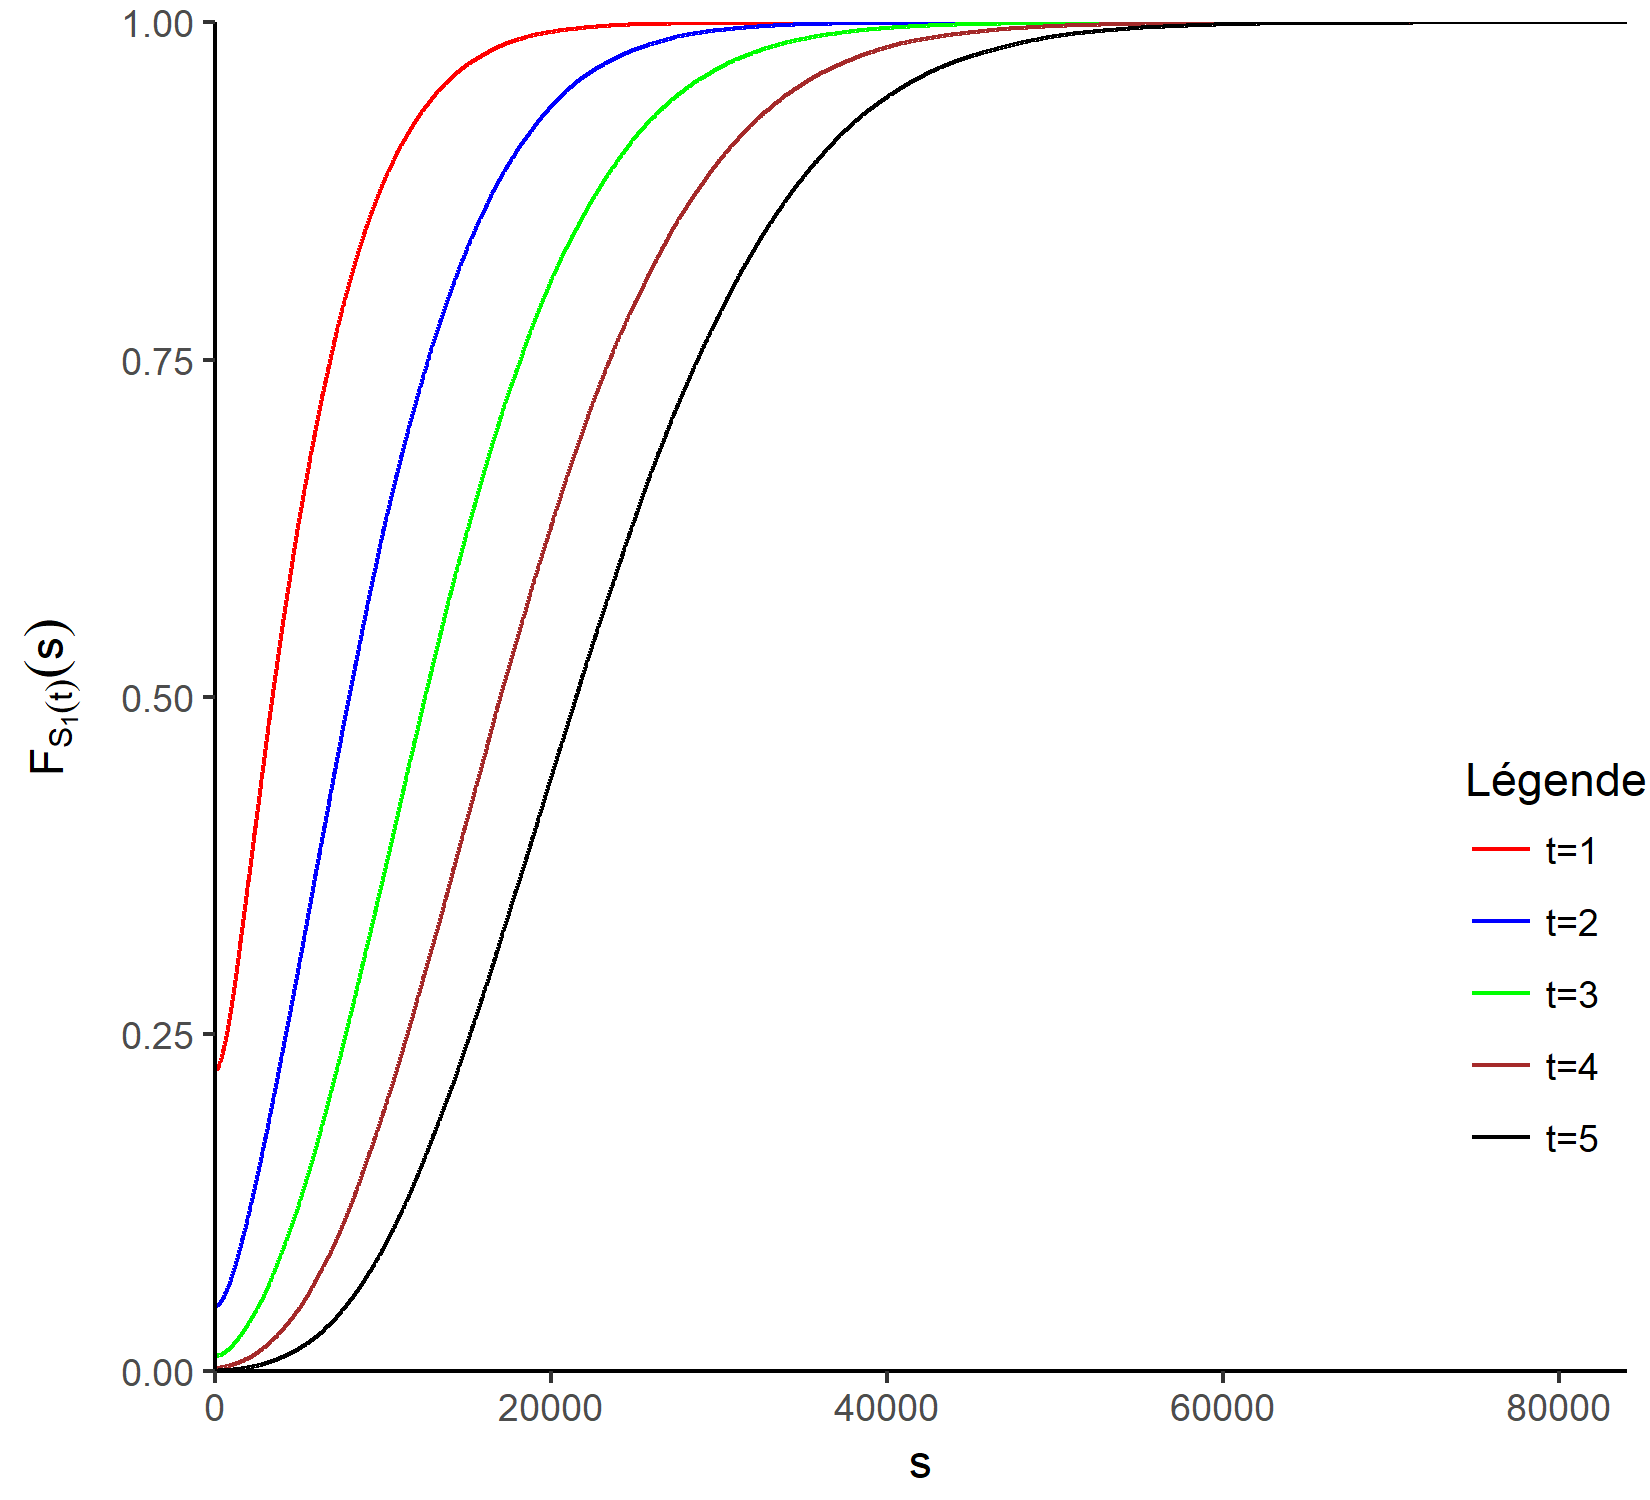
\includegraphics[scale=0.7]{Graphiques/empirique_Fn_S_1.png}
\end{figure}

\subsection*{B)}
\addcontentsline{toc}{subsection}{B)}

\hl{Équation VaR} \\
Le tableau \ref{TB:VaR processus 1} présente les valeurs simulées de la \emph{Value at Risk} (VaR) pour le 1\up{e} processus de poisson pour 3 différentes 
valeurs de $\alpha$. Comme observé dans la section précédante, plus l'intrervalle [0, t] augmente,
plus les valeurs sont en moyenne élevés du à l'augmentation de la fréquence. Il est donc encore logique, pour un même niveau $\alpha$, d'obtenir une VaR plus élévé 
pour une valeur de $t$ plus élevés. Le tableau \ref{TB:TVaR processus 1} présente les valeurs simulées de la \emph{Tail Value at Risk} (TVaR) pour le 1\up{e} processus 
de poisson pour 3 différentes valeurs de $\alpha$. L'avantage de cette mesure de risque est qu'elle donne une information sur la queue de la distribution.
Encore une fois, plus t augmente, plus la TVAR est grande. Le graphique \ref{GRAPH:Densite processus 1} permet de visualisé les queues des distributions qui 
augmente avec t. 

% latex table generated in R 3.4.1 by xtable 1.8-3 package
% Tue Nov 20 14:46:32 2018
\begin{table}[ht]
    \centering
    \caption{$VaR_\alpha\{S_1(t)\}$}
    \label{TB:VaR processus 1}
    \begin{tabular}{|cccccc|}
      \hline
      $\alpha$ & $t=1$ & $t=2$ & $t=3$ & $t=4$ & $t=5$ \\ 
      \hline
      95.0\% & 13320.86 & 20956.17 & 27909.60 & 34401.73 & 40614.64 \\ 
      97.5\% & 15795.33 & 24034.05 & 31485.11 & 38337.27 & 44959.93 \\ 
      99.0\% & 18774.93 & 27665.03 & 35879.80 & 43285.67 & 50109.22 \\  
       \hline
    \end{tabular} 
    \vspace{0.4cm}
    \caption{$TVaR_\alpha\{S_1(t)\}$}
    \label{TB:TVaR processus 1}
    \begin{tabular}{|cccccc|}
        \hline
        $\alpha$ & $t=1$ & $t=2$ & $t=3$ & $t=4$ & $t=5$ \\
        \hline
        95.0\% & 16743.80 & 25148.66 & 32847.72 & 39852.71 & 46492.07 \\ 
        97.5\% & 19070.86 & 27980.19 & 36193.06 & 43533.68 & 50452.44 \\ 
        99.0\%& 22091.67 & 31468.25 & 40415.74 & 48232.16 & 55239.44 \\ 
        \hline
    \end{tabular}
\end{table}


\begin{figure}[!ht]
    \centering
    \caption{Densité de $S_1(t)$}
    \label{GRAPH:Densite processus 1}
    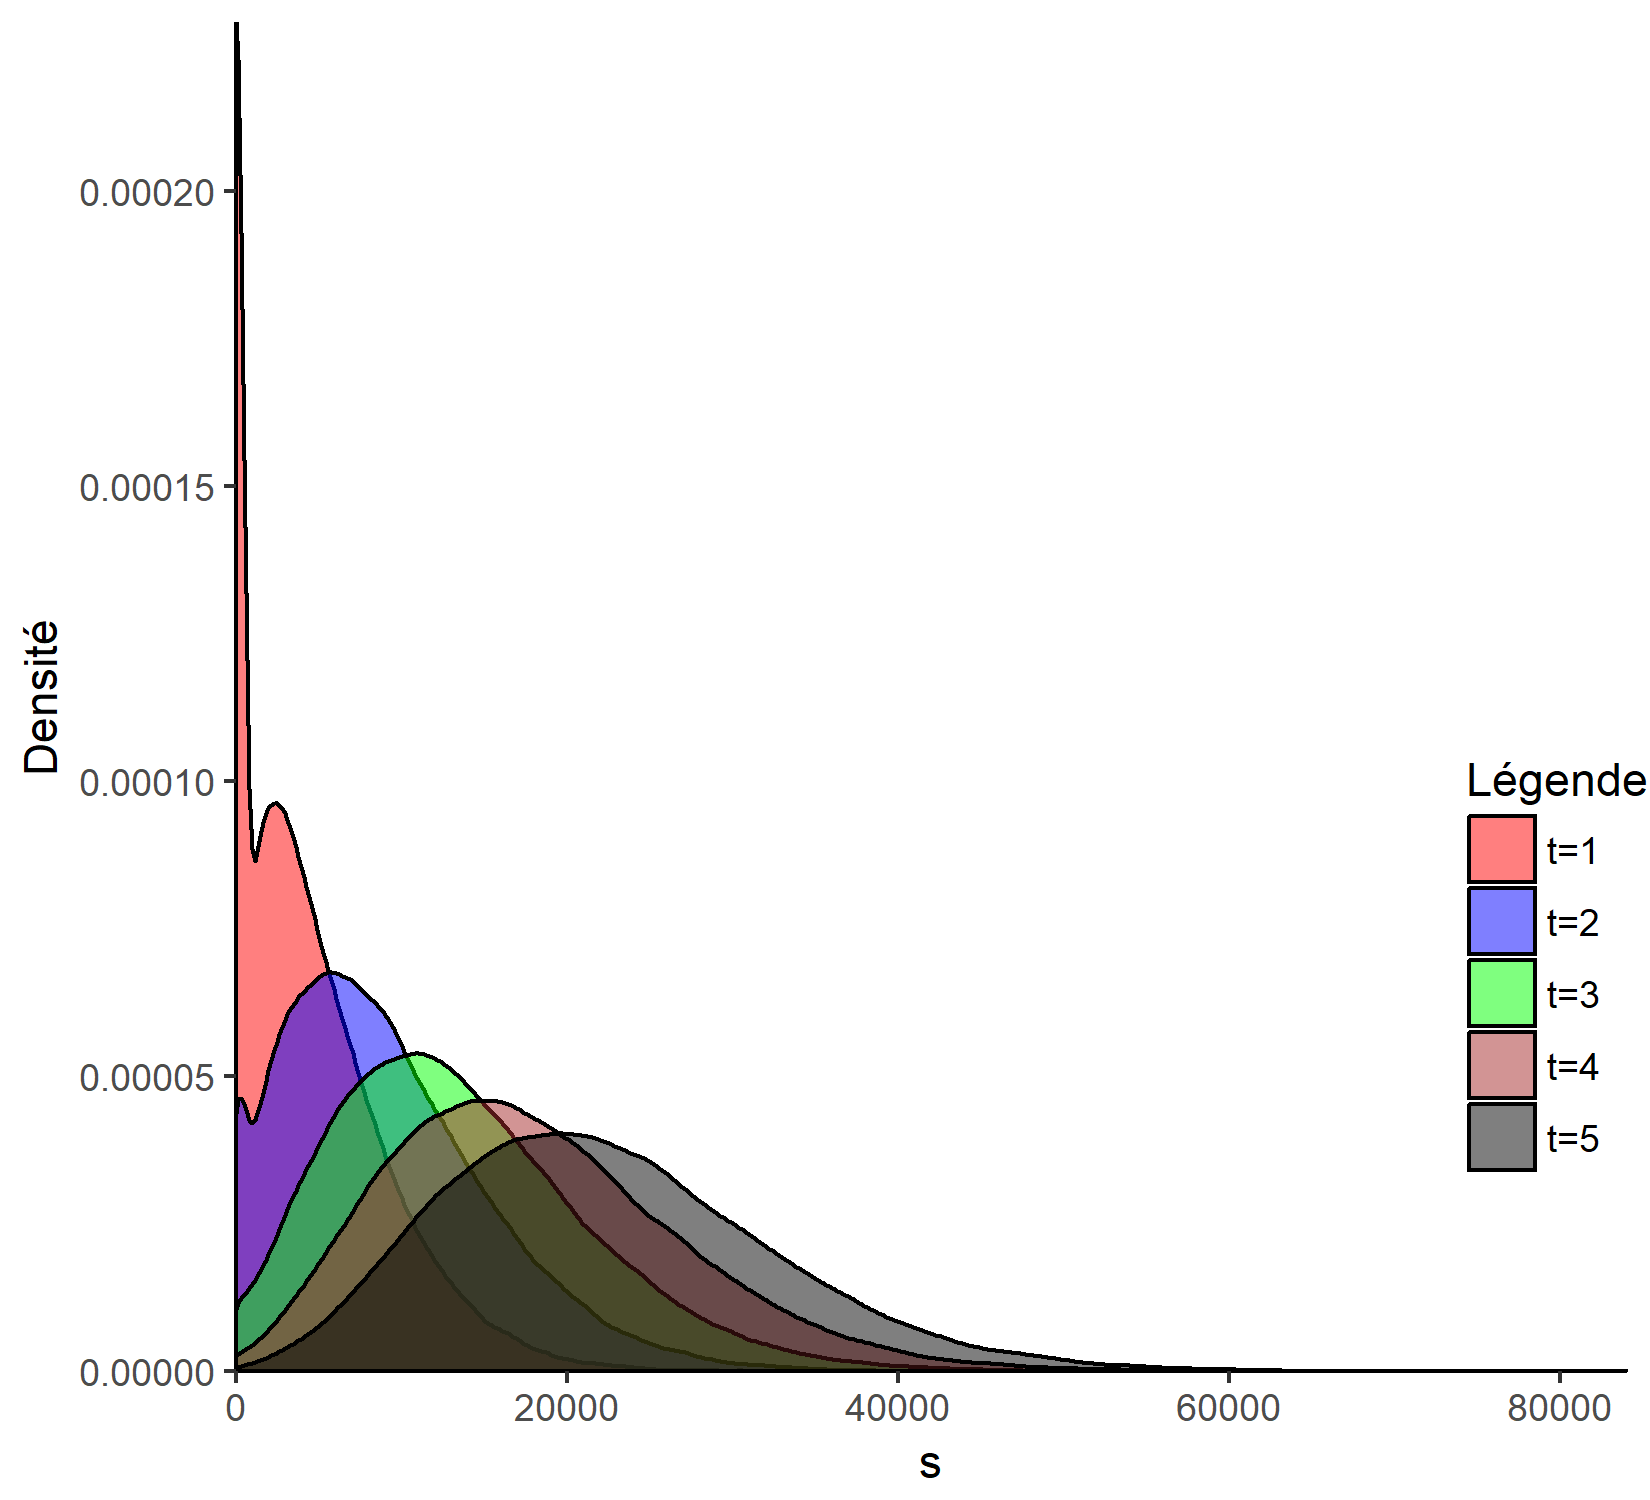
\includegraphics[scale=0.7]{Graphiques/densite_Fn_S_1.png}
\end{figure}




\chapter*{Question 2}
\addtocounter{chapter}{1}
\setcounter{section}{0}
\addcontentsline{toc}{chapter}{Question 2}
\section{}
\subsection*{A)}
\addcontentsline{toc}{subsection}{A)}

\subsection*{B)}
\addcontentsline{toc}{subsection}{B)}

\subsection*{C)}
\addcontentsline{toc}{subsection}{C)}

\section{}
\end{document}